\chapter{Soal}

%======================================================%
%                  TULIS SOAL DI SINI                  %
% Jangan Lupa untuk Menghapus Contoh Soal di Bawah Ini %
%======================================================%

Untuk bagian Soal, teks harus diambil dan disalin secara langsung dari naskah soal tugas. Penting untuk memastikan bahwa naskah soal tugas ini berasal dari jenis tutorial yang sudah Anda pilih. Setiap soal wajib disalin sama persis seperti yang tertera di naskah asli, kecuali untuk memperbaiki typo atau salah ketik yang mungkin ada. Akurasi dalam penyalinan soal adalah kunci untuk memastikan relevansi dan kejelasan dalam pengerjaan tugas Anda, sehingga tidak ada kerancuan dalam memahami instruksi.

Jika naskah soal berupa PDF yang berisi gambar, tabel, atau karakter yang sulit untuk ditulis ulang secara manual, Anda bisa mengakali hal ini dengan memilih salah satu cara berikut: 

\begin{enumerate}
    \item Menyisipkan file PDF tersebut secara langsung, kemudian memotong (\textit{crop}) bagian yang relevan dari gambar tersebut dan melampirkannya sebagai soal. Atau;
    \item Mengubah file PDF tersebut menjadi format gambar (seperti JPG, PNG, atau lainnya), kemudian memotong (\textit{crop}) bagian yang relevan dari gambar tersebut dan melampirkannya sebagai soal.
\end{enumerate}

Metode ini sangat membantu untuk menjaga keaslian visual dari soal yang sulit ditranskripsi, memastikan semua detail tersampaikan dengan baik.

\section{Contoh Soal yang Ditulis Kembali dari Naskah Soal}

Anda diminta untuk membuat sebuah dokumen LaTeX yang memamerkan kemampuan yang dapat dilakukan oleh LaTeX. Dokumen ini harus memuat kriteria berikut:

\begin{enumerate}[nosep]
    \item Struktur Dokumen
    \begin{itemize}[leftmargin=.62cm]
        \item Memakai \textit{document class report}.
        \item Sertakan halaman \textit{cover}.
        \item Sertakan nama Anda sebagai penulis.
        \item Sertakan tanggal/tahun pembuatan dokumen (gunakan perintah otomatis LaTeX).
        \item Berhubung \textit{document class report}, gunakan dua \textit{chapter} untuk membuat bagian Soal dan Jawaban.
        \item Penjeasan tentang struktur \textit{file} dokumen yang digunakan.
    \end{itemize}
    \item \textit{Heading} (\textit{Section} dan \textit{Paragraph})
    \item Jenis Font/Tulisan
    \item Penulisan Matematika
    \item Gambar
    \item Tabel
    \item Pengelolaan Daftar Pustaka
    \item Kutipan
\end{enumerate}

\section{Contoh Soal dari PDF}

Anda dapat meletakkan PDF naskah soalnya di dalam folder \verb|./pdf|, kemudian melampirkannya dengan: \\
\verb|\includegraphics[page=HALAMAN, trim=KIRI BAWAH KANAN ATAS]| \\
\verb|{LOKASI FILE}|

\noindent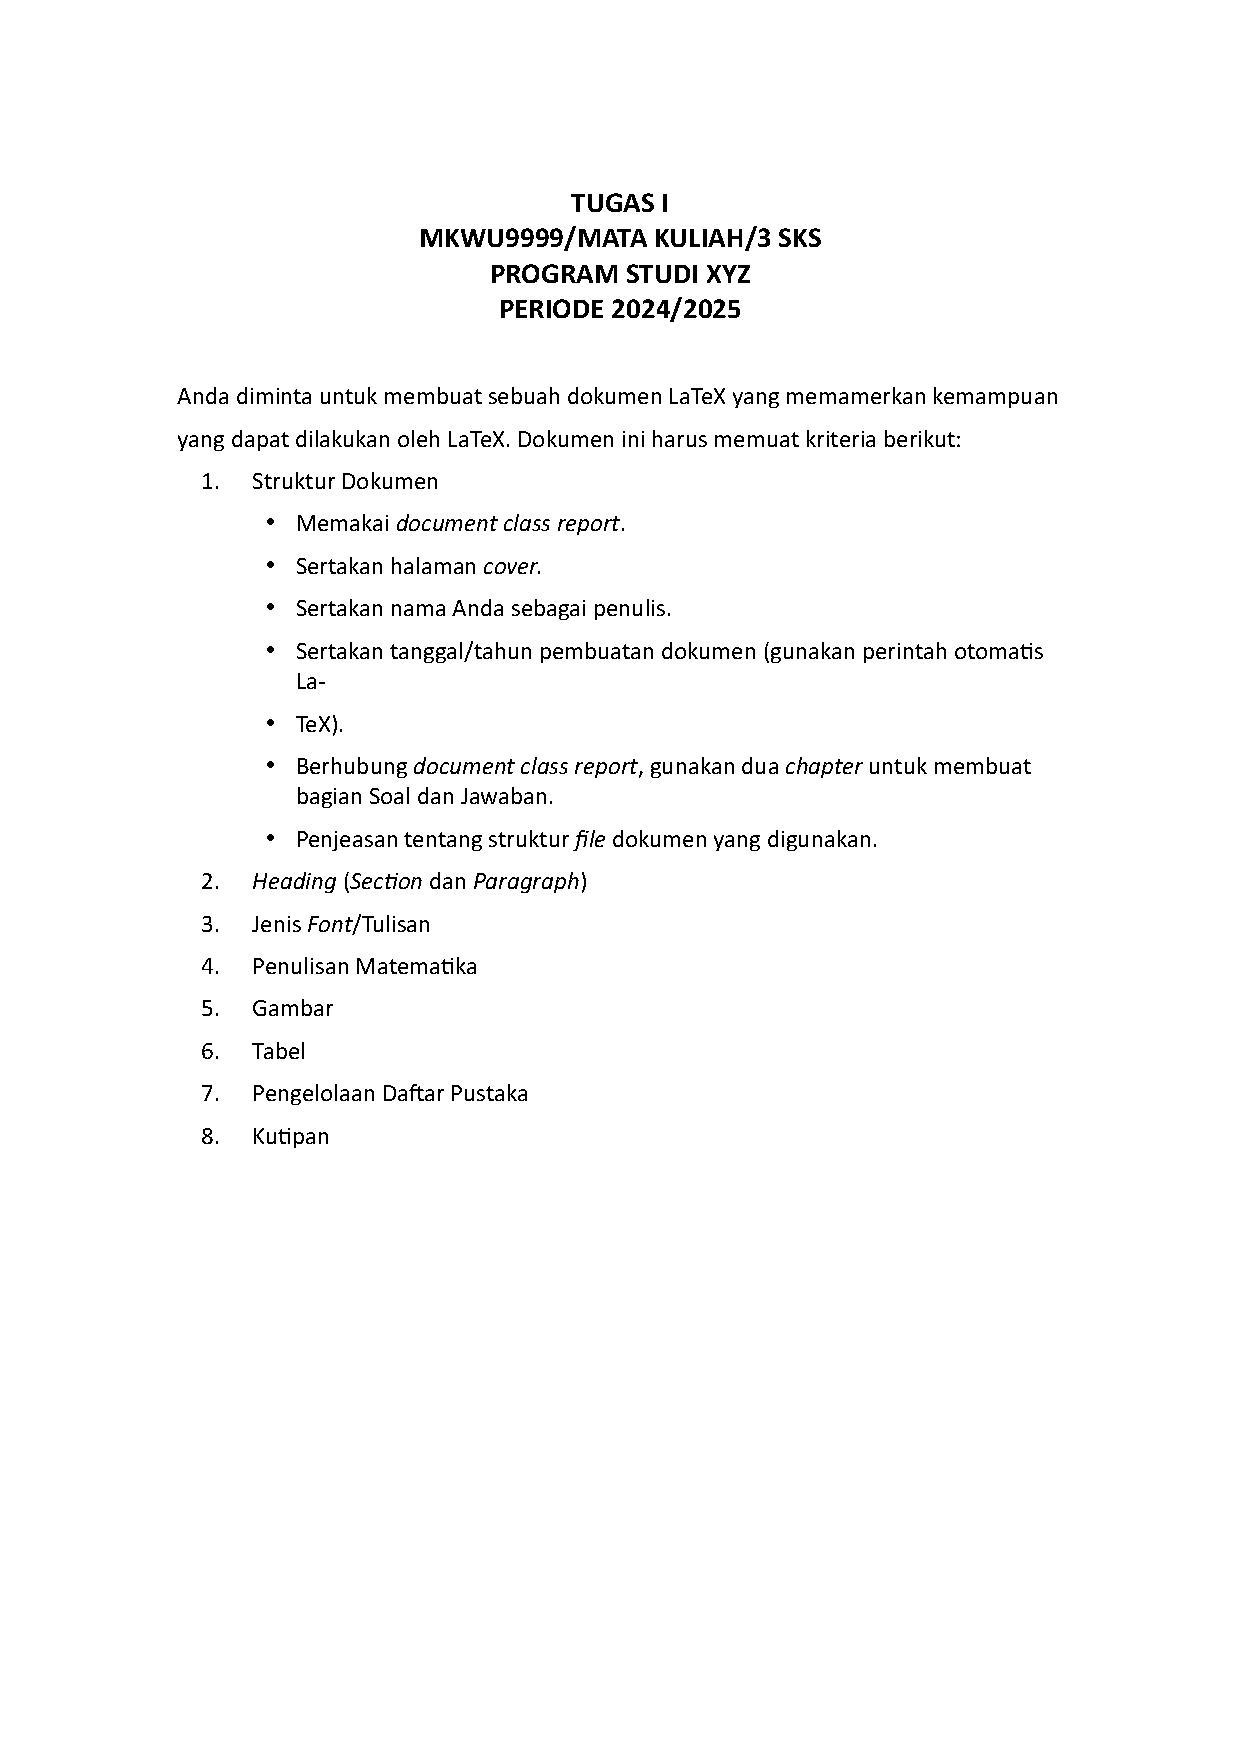
\includegraphics[page=1, trim=3cm 15cm 3cm 3cm]{pdf/Contoh Naskah Soal.pdf}